\documentclass[
	11pt,
	a4paper,
	% kosection,
	% footnote,
	% nobookmarks,
	% microtype,
	figtabcapt,
%	lwarp
]{oblivoir}

%%%%%%%%%%%%%%%%
% Front Matter %
%%%%%%%%%%%%%%%%

\setcounter{secnumdepth}{5} % section numbering depth


\usepackage[dvipsnames]{xcolor}

\usepackage{fapapersize}
\usefapapersize{*,*,30mm,*,35mm,*}
\definefageometry{default}{30mm,*,35mm,*}[\nopagecolor]
\definefageometry{test}{15mm,25mm,35mm,*}[\pagecolor{cyan!15}]


\usepackage{kotex-logo}

%for reference
\usepackage{hyperref}
\hypersetup{colorlinks=true, linkcolor=black, urlcolor=cyan}
\renewcommand{\figureautorefname}{그림~}
\renewcommand{\tableautorefname}{표~}
% \renewcommand{\sectionautorefname}{foobar}
% \renewcommand{\subsectionautorefname}{foobarbaz}

\usepackage{afterpage}
\usepackage{oblivoir-misc}
\usepackage{graphicx}
\usepackage{fancyvrb}

\usepackage{fontspec-xetex}
% \setmainhangulfont{NanumMyeongjo-YetHangul.ttf}

\usepackage{tabularx}


% for math fonts
\usepackage{amsmath}
\usepackage{amsthm}
\usepackage{amsfonts,amssymb}

% for citaiton
% \usepackage{biblatex}
							% Declare packages

%%%%%%%%%%
% Title, Authors, Date %
%%%%%%%%%%

\title{\vspace{-4cm}Week 1 : A Neural Probabilistic Language Model}
\author{120220210 고재현}
\date{\today}

\begin{document}

%%%%%%%%%%
% covers %
%%%%%%%%%%


%%%%%%%%%%%%%%%%%%%%%
% Table of Contents %
%%%%%%%%%%%%%%%%%%%%%
\maketitle

% \begin{abstract}
% 이 문서는 2022 인공지능개론(EEE4178) 과목의 설명서이다.

% \end{abstract}

\pagenumbering{roman}                           % Start page numbering in Roman numerals
% \tableofcontents*        						% Add table of contents
% \clearpage

%%%%%%%%%%%%%%%%%
% preliminaries %
%%%%%%%%%%%%%%%%%

\setcounter{table}{0}		                    % Reset table counter
\setcounter{figure}{0}		                    % Reset figure counter

%%%%%%%%%%%%%
% Main Text %
%%%%%%%%%%%%%

\pagenumbering{arabic}							% Start page numbering in Arabic numerals

\section{Introduction}
사람이 문장을 구성하는 단계를 생각해 보자. 중심이 되는 단어를 생각하고, 그 단어들을 조합하여 문장을 구성한다.
또는, 완성된 문장에서 특정 요소를 교체하여 문장을 완성하기도 한다.
이러한 언어 시퀀스의 구성 방식을 컴퓨터가 수행할 수 있는 반복 가능한 형태(Algorithmic)로 만드려면 어떻게 해야 할까?

\section{related works}
\subsection{Probabilistic Language models}
인간이 언어를 학습하는 과정을 문장의 요소 간, 혹은 단어의 요소 간의 관계를 확률적으로 표현하는 방법을 배우는 것이라고 한다면,
이러한 확률 관계를 잘 모델링 할 수 있다면 인간의 학습 과정을 재현할 수 있을 것이다.
이러한 관점에서 출발한 것이 바로 통계적 언어 모델(Probabilistic language modeling) 이다.
이는 문자, 단어, 문장 등의 언어 토큰 시퀀스가 주어졌을 때,
다음에 나올 토큰의 확률을 예측하는 기법이다.
수업 시간에는 주로 단어 단위의 시퀀스를 다루었으나, 목적에 따라 시퀀스의 단위는 달라질 수 있다.
이러한 확률 모델들 중에 가장 유명하고 간단한 형태인 N-gram model 을 다루어 본다.\footnote{논문에서 또한 다루었다.}

\subsection{N-gram models}
n-gram 모델은 통계적 언어 모델링에서 가장 기본적인 방법 중 하나로,
연속된 $n$개의 단어를 하나의 단위로 취급하여 각 단어가 다음 단어로 등장할 확률을 추정하는 모델이다.

\begin{equation}
	P(w_n | w_{n-1}, w_{n-2}, ..., w_1) = P(w_n | w_{n-1}, w_{n-2}, ..., w_{n - n_{gram} + 1})
\end{equation}

예를 들어 bigram model을 생각하자.
The cat sat on the mat
이라는 문장이 주어졌을 때, bigram model은 문장을 $P(The), P(cat|The), P(sat|cat), P(on|sat), P(the|on), P(mat|the)$ 로 분리된 조건부확률의 chain으로 보고,
각각의 확률을 corpus에서 빈도수를 통해 미리 계산해둔 뒤 이를 꺼내어 문장의 생성 확률을 계산한다.
이를 위해서는 말뭉치 내의 모든 단어의 빈도를 구하여 조건부 확률표를 구성해야 한다. 또한, 긴 범위의 문맥을 고려하기 어렵다는 단점이 있다.

\section{Neural Probabilistic Language Model}
Neural Probabilistic Language Model\cite{bengio2003neural}은 N-gram model을 neural network로 구현한 모델이다.
\begin{figure}[htp]
	\centering
	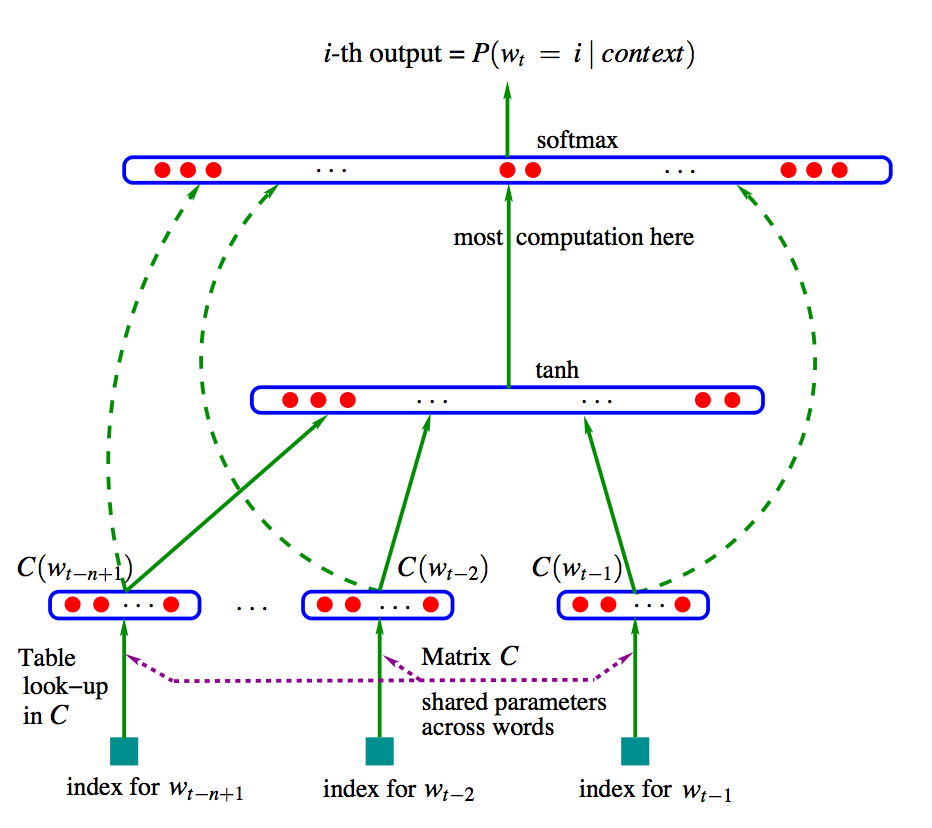
\includegraphics[width=0.5 \textwidth]{figures/NPLM.png} 
	\caption{NPLM Architecture}
	\label{fig:NPLM}
\end{figure}
\subsection{forward propagation}
먼저, 말뭉치 내의 각각의 단어를 one-hot encoding하여 벡터로 표현한다. 이를 $w_1, w_2, ..., w_n$ 이라고 하자.
이제 단어 두 개가 주어졌다고 하자. 예를 들어 '나는', '학교에' 이다. 여기에서 '간다' 라는 one-hot vector를 추론하는 것이 모델의 목표이다.
이를 수식으로 표현하면 다음과 같다.
\begin{equation}
	 P(w_t | w_{t-1}, w_{t-2}, ..., w_{t - n + 1}) = \frac{\exp(y_{w_t})}{\sum_{i=1}^n \exp{(y_i)}}
\end{equation}
단어들의 관계를 표현하기 위해 one-hot vector들을 열백터로 변환하는 행렬 $C$를 정의한다.
이를 통해 $w_1, w_2, ..., w_n$ 사이의 관계를 반영하여 $Cw_1, Cw_2, ..., Cw_n$ 으로 표현할 수 있다.
이제 각각의 변환된 단어를 이어붙여 하나의 벡터로 표현하고, 이를 $x_t$ 라고 하자.
이어붙이는 이유는 단어들의 정보를 잃어버리지 않고, 단일 백터로 만들어 2-layer neural network를 통과시키기 위함이다.
그리고 2-layer network를 통해 출력 단어 $y$를 예측한다. 모델은 단순한 2-layer perceptron이다.
\begin{equation}
	y_{wt} = b + U \cdot \tanh(d + Hx_t)
\end{equation}
출력을 softmax 함수를 통과시켜 확률로 변환한다.

\subsection{bacpropagation}
forward propagation의 출력과 실제 단어의 임베딩 값을 비교(negative log likelihood loss)하여 역전파를 통해
임베딩 변환 행렬 $C$ 및 네트워크 파라미터를 학습한다.

\subsection{result}
결과는 perplexcity 측면에서 기존 언어 모델보다 강점을 보여주고 있다.
이 논문에 출판될 당시에는 연산능력 측면에서 한계가 있었으나, 현재는 GPU를 이용하여 재현하면 금새 구현 가능할 것이다.
\begin{figure}[htp]
	\centering
	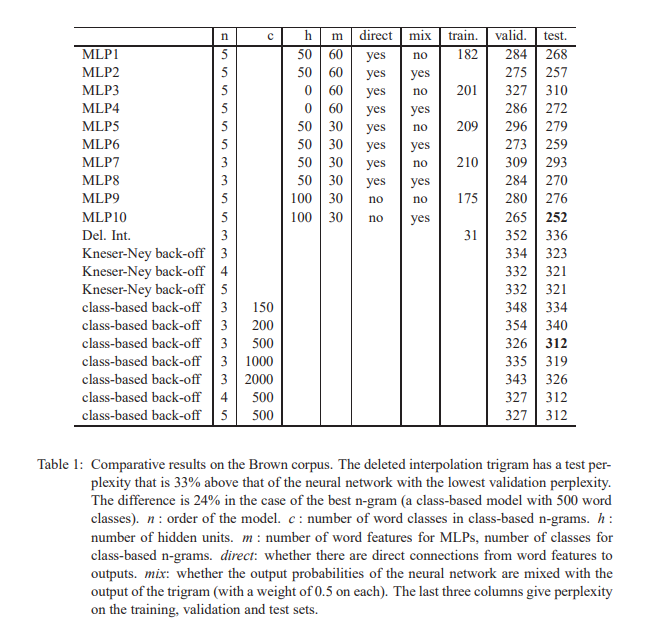
\includegraphics[width=\textwidth]{figures/NPLM_result.png} 
	\caption{NPLM result}
	\label{fig:NPLM}
\end{figure}
%%%%%%%%%%%%%%%%%%%%%%
% References Section %
%%%%%%%%%%%%%%%%%%%%%%
\bibliographystyle{ieeetr}						% Declare bibliography style
\bibliography{week2.bib}							% Declare bibliography file

\clearpage

\end{document}
